\documentclass[11pt]{amsart}
%basic packages and commands
\usepackage{amsmath,amsthm,amssymb,eufrak}
\usepackage{hyperref}
\usepackage{xcolor}

\newcommand{\bb}[1]{\mathbb{#1}}
\newcommand{\mbf}[1]{\mathbf{#1}}
\newcommand{\fr}[1]{\mathfrak{#1}}
\renewcommand{\mod}{\text{ mod }}
\renewcommand{\bar}[1]{\overline{#1}}

%theoremstyles
\usepackage{thmtools}
\declaretheorem[style=plain, numberwithin=section, name=Theorem]{theorem}
\declaretheorem[style=plain, sibling=theorem, name=Corollary]{cor}
\declaretheorem[style=plain, sibling=theorem, name=Proposition]{prop}
\declaretheorem[style=plain, sibling=theorem, name=Lemma]{lemma}

\declaretheorem[style=definition, sibling=theorem, name=Definition]{defi}
\declaretheorem[style=definition, numbered=no, name=Example]{ex}
\declaretheorem[style=remark, sibling=theorem, name=Remark]{remark}

%bibliography
\usepackage[style=alphabetic, citestyle=alphabetic, backend=biber]{biblatex}
\renewbibmacro{in:}{}
\addbibresource{refs.bib}

%layout
\usepackage[margin=4cm]{geometry}
%\usepackage{titlesec}


\title{The Law of Quadratic Reciprocity}
\author{Niels Ketelaars}
\begin{document}
\maketitle
\section{Introduction}
\pagenumbering{arabic}
{\hypersetup{linkcolor = black}

  The law of quadratic reciprocity is one of the most famous and important results from number theory. Known already to mathematicians like Euler and Legendre, it wasn't until the start of the 19th century when Gauss gave the first (complete) proof, who called it his \emph{theorematis fundamentalis} (see also Figure \ref{fig:gauss}). Near the end of the 19th century, many more proofs were known, and a large part of algebraic number theory was concerned with finding generalizations, to gain a deeper understanding of the theorem.
  Below we first give a short historical outline and motivation, after which we will give a proof based on one of Gauss's proofs. Finally we will discuss the theorem in the context of modern algebraic numebr theory, and mention a few generalizations. 
\begin{figure}[H]
\centering
\label{fig:gauss}
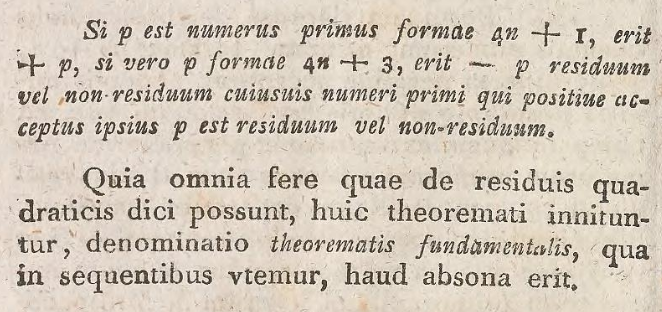
\includegraphics[width=10cm]{gauss.png}
\caption{Gauss's original formulation\protect\footnotemark from \cite{cfg}.}
\end{figure}
\footnotetext{\label{ftn:gauss}``If $p$ is a prime number of the form $4n+1$, then $p$, or if $p$ is of the form $4n+3$, then $-p$, will be a residue, respectively a non-residue, of those primes, that are, when positive, a residue, respectively a non-residue of $p$ itself."}

}

\section{Fermat, Euler and Legendre}
This section is largely based on the first few chapters of David Cox's book \cite{cox}. For proofs of the claims in this sections and additional information we point the reader to this book.

The history of quadratic reciprocity begins with a famous result of Fermat, that seems unrelated at first.
\begin{theorem}[Fermat]
  Let $p$ be an odd prime. Then there exist integers $x,y$ with $p=x^2+y^2$ if and only is $p\equiv 1 \mod 4$.
\end{theorem}
It is fairly unexpected that the primes which can be written as a sum of squares can be characterized by their residue class modulo $4$.
A natural generalization is to consider for fixed $n\in \bf Z$, which primes can be written as $x^2+ny^2$, and in particular we wonder if these primes can again be characterized by their residue class modulo some fixed number.
This question was examined by Fermat and Euler among others. Euler quickly realized Fermat's original theorem had to do with the fact that $-1$ is a square in $\bf Z/p\bf Z$ if and only if $p\equiv 1\mod 4$. For our more general problem, is is therefore natural to consider for which primes we have that $-n$ is a square modulo $p$. This was Euler's motivation to study squares in $\bf Z/p\bf Z$, and it is how he eventually stumbled across the law of quadratic reciprocity. He noticed that for two odd primes $p$ and $q$, there was a relation between whether $p$ is a square modulo $q$, and whether $q$ is a square modulo $p$. Before we state the theorem in full, we need some notation due to Legendre.
\begin{defi}
For $t\in \bf Z$ and $p$ an odd prime, the \emph{Legendre symbol} is
\[\leg tp \deff  \begin{cases} 0 &\text{if } p|t, \\ 1 &\text{if } p\nmid t \text{ and } t \text{ is a square mod } p, \\ -1 &\text{if } p\nmid t \text{ and } t \text{ is not a square mod } p. \end{cases}\]
\end{defi}
Before we continue we note some nice properties of the Legendre symbol.

\begin{prop}
\label{prop:leg}
For $a,b \in \bf Z$, we have that
\begin{enumerate}
\item $\leg{ab}{p} = \leg ap \leg bp$;
\item $\leg ap \equiv a^{\frac{p-1}{2}} \mod p$;
\item $\leg {-1}{p} = (-1)^{\frac{p-1}{2}}$.
\end{enumerate}
\end{prop}
These properties will become very important later on; in fact, the second is so fundamental that it was Legendre's original definition of the symbol.

\begin{remark}
  \label{rem:hom}
  As a consequence of Proposition \ref{prop:leg}, the Legendre symbol induces a homomorphism $(\bf Z/p\bf Z)^* \to \{\pm 1\}$ given by $a \mod p \mapsto\leg ap$. It is surjective, and its kernel is precisely the set of squares. Thus the set of squares forms a subgroup of index 2, from which it follows that there are as many squares as non-squares in $(\bf Z/p\bf Z)^*$. This will become important later in the proof of Lemma \ref{lem:tau}.
\end{remark}

We can know present the theorem in its most common form.

\begin{theorem}[Quadratic Reciprocity]
\label{thm:qr}
Let $p,q$ be distinct odd primes. Then we have that
\[\leg qp = \leg pq (-1)^{\frac{p-1}{2} \frac{q-1}{2}}. \]
\end{theorem}

The fact that there is any relation at all between whether $p$ is a square modulo $q$ and whether $q$ is a square modulo $p$ is incredibly unexpected and remarkable. Paired with the fact that the theorem is incredibly easy to state, many consider it one of the most beuatiful theorems in number theory.

If we write \[p^* \deff \leg{-1}{p} p = (-1)^{\frac{p-1}{2}} p,\] it follows from Proposition \ref{prop:leg} that the above formulation is equivalent to saying that $\leg qp = \leg{p^*}{q}$. This is the formulation that is most commonly found in algebraic number theory, and it is the one we will prove below.

\section{Gauss and quadratic reciprocity}
The proof we give in this section is largely based on Gauss's sixth proof, and can be found in the well-known book of Ireland and Rosen \cite[Chapter 6, p. 70]{ir}. Recall that a \emph{primitive n-th root of unity} is a complex number $\zeta$ satisfying $\zeta^n=1$ and $\zeta^k\neq 1$ for $1\leq k < n$. For the remainder of this article, $\zeta$ will be be a fixed primitve $p$-th root of unity. We start with a lemma about these roots of unity.

\begin{lemma}
\label{lem:pew}
Let $c\in \bf Z$. Then
\[ \sum_{t=0}^{p-1} \zeta^{ct} = \begin{cases} p &\text{if } p|c, \\ 0 &\text{otherwise.} \end{cases} \]
\end{lemma}
\begin{proof}
If $p|c$, we have $\zeta^{ct}=1$ for all $t$, and hence the sum is equal to $p$. 
Otherwise we see that
\[\sum_{t=0}^{p-1} \zeta^{ct} = \frac{\zeta^{cp}-1}{\zeta^c-1} = 0.\qedhere \]
\end{proof}

\begin{defi}
For $a\in \bf Z$, the \emph{quadratic Gauss sum} is
\[\tau_a \deff \; \sum_{t=0}^{p-1} \leg tp \zeta^{at} .\] We write $\tau = \tau_1$.
\end{defi}
At first this may seem like a rather arbitrary definition. Intuitively one can think about it as a way of encoding all different Legendre symbols of $p$ into a single number. This becomes more clear in the following lemma.

\begin{lemma}
\label{lem:tau}
$\tau_a = \leg ap \tau$.
\end{lemma}

\begin{proof}
In the case that $a$ is a multiple of $p$, the right hand side is equal to 0. We also have that $\zeta^{at}=1$ for all $t$, thus  \[\tau_a = \sum_{t=0}^{p-1} \leg tp,\] and this is indeed $0$ because of Remark \ref{rem:hom}, saying there are as many squares as non-squares in $(\bf Z /p\bf Z)^*$.

If $p\nmid a$, we have $\leg{a}{p}^2=1$, so
\[ \tau_a = \sum_{t=0}^{p-1} \leg tp \zeta^{at} =\leg{a}{p}^2 \; \sum_{t=0}^{p-1} \leg {t}{p} \zeta^{at}= \leg{a}{p}\sum_{t=0}^{p-1} \leg {at}{p} \zeta^{at},\] 
where the last equality follows from the multiplicativity of the Legendre symbol (Proposition \ref{prop:leg}).
Now note the following: if $t$ runs through a system of representatives of $\bf Z /p\bf Z$, then so does $s=at$. Thus
\[\leg{a}{p}\sum_{t=0}^{p-1} \leg {at}{p} \zeta^{at}=\leg ap \sum_{s=0}^{p-1} \leg {s}{p} \zeta^{s} = \leg ap \tau.\qedhere\]
\end{proof}

We now arrive at what is probably the most important ingredient of the proof of quadratic reciprocity.
\begin{prop}
\label{prop:pst}
$\tau^2 = p^*$.
\end{prop}

\begin{proof}
The main idea is to write the sum $\sum_{a=0}^{p-1} \tau_a \tau_{-a}$ in two different ways, and then setting these two expressions equal. Using Lemma \ref{lem:tau} we get that for $p\nmid a$, we have $\tau_a \tau_{-a} = \leg ap \leg {-a}{p} \tau^2 = \leg {-1}{p} \tau^2$, and hence we see that
\[\sum_{a=0}^{p-1} \tau_a \tau_{-a} = \leg {-1}{p}(p-1) \tau^2. \]
On the other hand the definition of $\tau_a$ gives us that 
\[\sum_{a=0}^{p-1} \tau_a \tau_{-a} = \sum_{a=0}^{p-1} \sum_{x,y=0}^{p-1} \leg xp \leg yp \zeta^{ax}\zeta^{-ay} = \sum_{x,y=0}^{p-1} \leg{x}{p}\leg{y}{p} \sum_{a=0}^{p-1} \zeta^{a(x-y)}.\]
By Lemma \ref{lem:pew} the inner sum is equal to 0 for $x\neq y$, and otherwise it is equal to $p$. Thus we can rewrite the double sum over $x$ and $y$ as a single sum over $x$, by replacing all instances of $y$ with $x$, since the terms for which $x\neq y$ are zero. What remains is
\[\sum_{x,y=0}^{p-1} \leg{x}{p}\leg{y}{p} \sum_{a=0}^{p-1} \zeta^{a(x-y)}=\sum_{x=0}^{p-1} \leg{x^2}{p} p = (p-1)p.\]From this we see that we must have $ \leg {-1}{p}(p-1) \tau^2 = (p-1)p$, or put differently $\leg {-1}{p}\tau^2 = p$. Lastly we can multiply this equality by $\leg{-1}{p}$, to arrive at the fact that \[\tau^2 = \leg{-1}{p} p.\qedhere \]
\end{proof}

At last, we are ready to give the proof of the law of quadratic reciprocity.
\begin{proof}[Proof of Theorem \ref{thm:qr}]
We will use the same general idea as the previous proof, and express $\tau^{q+1}$ in two ways. On one hand, 
\[\tau^{q+1} = (\tau^2)^{\frac{q-1}{2}} \tau^2 = (p^*)^{\frac{q-1}{2}} p^* \equiv \leg{p^*}{q}p^* \mod q, \] where we used Proposition \ref{prop:pst} for the second equality, and part 2 of Proposition \ref{prop:leg} for the last congruence.

On the other hand, we can write out that
\[\tau^{q+1} = \left( \sum_{t=0}^{p-1} \leg tp \zeta^{t} \right)^q \tau. \]
If we were to expand this using repeated binomial expansion, we would certainly get all the individual terms of the sum raised to the power $q$, plus a number of cross terms. Since $q$ is prime, one can easily show are binomial coefficients $\binom{q}{k}$ are divisible by $q$ for $1<k<q$. Hence the coefficients of the cross terms are divisible by $q$. If we therefore consider the entire expression modulo $q$, we are left with 
\[\tau^{q+1} \equiv \left( \sum_{t=0}^{p-1} \leg{t}{p}^q \zeta^{qt} \right) \tau = \tau_q \tau=  \leg qp \tau^2 = \leg qp p^* \mod q ,\]
where the last two equalities follow from Lemma \ref{lem:tau} and Proposition \ref{prop:pst} respectively. Thus we see that $\leg qp p^* \equiv \leg{p^*}{q}p^* \mod q$, and because $p$ and $q$ are distinct, $p^*$ is invertible mod $q$, and hence $\leg qp \equiv \leg{p^*}{q} \mod q$. Finally, because -1 and 1 are never congruent   modulo an odd prime, we get that $\leg qp = \leg{p^*}{q}$.
\end{proof}
The careful reader may have noticed we are working modulo $q$ while our expressions can contain complex numbers. Using facts about rings one can easily show that this is still valid.\footnote{We are in fact working in the ring $\bf Z[\zeta]/(q)$.}

\section{Artin and Langlands}
After Gauss had given this proof in 1818, many number theorists were convinced there was something deeper going on in the proof. The connection with roots of unity in particular, that is nowhere to be found in the theorem itself, is plainly clear in the proof. 
This was one of the main reasons for the beginning of \emph{class field theory}, a subfield of algebraic numebr theory, dealing mainly with so called Abelian extensions of number fields and generalizations of the classical reciprocity law.
One of the highlights of class field theory was the proof at the start of the 20th century of the \emph{Artin reciprocity law}. This theorem, which to this day is still one of the most important results in number theory, makes it possible to place quadratic reciprocity and Gauss's proof in a broader context, making it possible to gain a much more deep understanding. We refer the interested reader to the accessible article of Lenstra and Stevenhagen \cite{hlps}.

In modern number theory, the Langlands program is a central object of study. It is a collection of conjectures that can in a way be seen as the `ultimate' generalization of quadratic reciprocity. Both the aforementioned theorem of Artin, but also the modularity theorem, which was the basis for Wiles's proof of Fermat's Last Theorem, are special cases of Langlands's conjectures. In 2018 Robert Langlands won the Abel prize for his work. See for instance \cite{as} for a short and accessible introduction.

The law of quadratic reciprocity thus may seem simple, and is probably nothing more than a cool party trick at first. Nevertheless, there is a lot of beautiful mathematics behind it, and it would be difficult to say were number theory as a whole would currently be if it hadn't been discovered.

\addcontentsline{toc}{section}{Referenties}
\printbibliography


\end{document}